\section{Обзор литературы}
\label{sec:domain}

\subsection{Обзор основных понятий 3D графики}
\label{sub:domain:overview_3d}
3D компьютерная графика -- способ представления геометрической информации в трехмерном пространстве (зачастую представленной
в Декартовой системе координат), сохраненной на компьютере с целью произведения вычислений и создания двухмерных изображений.
Результирующие изображения могут быть в сохранены для просмотра в будущем, либо отображаться в реальном времени. 

Процесс отображения 3D графики основан на многих алгоритмах работы с двухмерными векторными изображениями в стадии обработки
каркасов моделей (также называемых wireframe-моделями) и алгоритмах работы с растровой графикой при получении финального изображения.
Зачастую, из-за смешанного подхода к работе с трехмерной графикой, сложно выделить набор явных различий между 3D и 2D, так как многие
среды, предназначенные для работы с двухмерной графикой используют техники обработки трехмерных изображений (например, для достижения
реалистичной модели освещения), а системы работы с трехмерной графикой подразумевают использования техник обработки двухмерных изображений
(например, постобработка).

Понятие объектов трехмерной графики часто отождествляют с понятием 3D моделей, однако эти понятия не совсем тождественны,
так как модель по своей сути является лишь математическим представлением трехмерного объекта. Она не является производной
компьютерной графики до тех пор, пока не будет отображена на двухмерном изображении. Модель может быть отображена на изображении
в результате процесса, называемого <<3D-рендеринг>>, а также использована во всевозмжных не графических симуляциях либо вычислениях.
Еще одним применением трехмерных моделей, набирающим популярность в последние годы, можно называть 3D-печать. В случае трехмерной
печати, модель отображается из математического представления в реальный физический объект, однако, с некоторыми ограничениями, в
основном связаннными с предельной точностью печати.


\subsection{Обзор основных понятий 3D моделирования}
\label{sub:domain:overview_3d_modelling}
В контексте трехмерной компьютерной графики, 3D-моделированием (либо трехмерным моделированием) называют процесс разработки
математического представления трехмерной поверхности объектов (живых либо неживых по своей природе) с использованием специальных
инструментов. Продукт трехмерного моделирования -- 3D-модель объекта. Результирующая трехмерная модель может быть отображена
на двухмерном носителе либо напечатана с помощью 3D-принтера либо использована в компьютерной симуляции.

Модели могут быть созданы в автоматическом режеми либо вручную. Процесс ручного создания трехмерной модели по своей сущности
схож с процессом создания скульптуры.

Программное обеспечение трехмерного моделирования, известное под названием 3D-модельер - категория графических приложений, использующихся для создания трехмерных
моделей.

% - Представление моделей
Практически все трехмерные модели могут быть условно поделены на две основные категории.
Цельные -- данные модели определяют объем объекта, который они представляют. Цельные модели в основном используются в инжеренрых и медицинских симуляциях
и обычно строятся с помощью геометрических примитивов.\cite{solid_modelling}

Оболочечные либо поверхностные -- данные модели представляют поверхность объекта (например, сферу шара, либо бесконечно тонкую яичную скорлупу).
Основная область применения таких моделей -- игровая и киноиндустрия, визуализация данных.

Цельные и поверхностные модели функциональ представляют идентичные объекты. Разница между ними в основном состоит в том, каким образом они
определяются и редактируются, а так же набор соглашений используемых при работе с такими моделями, например -- правила и типы аппроксимации
при вычислениях. 

Поверхностные модели должны быть непрерывными (то есть не иметь отверстий, трещин в оболочке) для того чтобы использовать их в
качестве натурального объекта. Полигональные сетки (и, в несколько меньшей степени, подразделенные поверхности) являются наиболее широко распространенной
категорией поверхностных моделей. Горизонтально выровненные наборы полигонов являются полезным инструментов в представлении видоизменяющихся или
деформирующихся поверхностей, подверженных большому числу топологических изменений, таких как, например, поверхность жидкости.

Процесс трансформации представления объектов, например, таких как координаты цетральной точки сферы и ее радиуса, в полигональное представление называется тесселяцией.
Этот процесс генерирует полигональный рендеринг, в котором объекты представленные в виде абстрактных фигур (называемые примитивами - сферы, конусы и т.п) 
преобразуются в полигональные меши, состоящие из сети взаимосвязынных треугольников. 

Меши, существующие в виде треугольников, гораздо популярнее, нежели меши основанные из квадратах, 
потому что было доказано, что они легче поддаются растеризации (поверхность, описываемая каждым треугольником, является плоской, поэтому проекция всегда выпукла).
Полигональное представление не всегда используется в процессе рендеринга, и в этих случаях тесселяция не включена в преобразование из абстрактного представления в конечный результат рендеринга.

% - Процесс моделирования
Существует три популярных пути представления модели:

1) Полигональное моделирование 
Вершины в трехмерном пространстве, называемые вертексами, соединенные отрезками прямых, формирует полигональную сеть.
Подавляющее большинство существующих трехмерных моделей на сегодня основано на текстурированных полигональных моделях, из-за их гибкости
и возможности компьютеров использовать сплайновое моделирование.
%Polygonal modeling – Points in 3D space, called vertices, are connected by line segments to form a polygon mesh. The vast
%majority of 3D models today are built as textured polygonal models, because they are flexible and because computers can
%rurve modeling – Surfaces are defined by curves, which are influenced by weighted control points. The curve follows (but
%does not necessarily interpolate) the points. Increasing the weight for a point will pull the curve closer to that point.
%Curve types include nonuniform rational B-spline (NURBS), splines, patches, and geometric primitives
%Digital sculpting – Still a fairly new method of modeling, 3D sculpting has become very popular in the few years it has
%been around.[citation needed] There are currently three types of digital sculpting: Displacement, which is the most widely
%sed among applications at this moment, uses a dense model (often generated by subdivision surfaces of a polygon control
%mesh) and stores new locations for the vertex positions through use of an image map that stores the adjusted locations.
%Volumetric, loosely based on voxels, has similar capabilities as displacement but does not suffer from polygon stretching
%when there are not enough polygons in a region to achieve a deformation. Dynamic tessellation is similar to voxel but divides
%the surface using triangulation to maintain a smooth surface and allow finer details. These methods allow for very artistic
%exploration as the model will have a new topology created over it once the models form and possibly details have been sculpted.
%The new mesh will usually have the original high resolution mesh information transferred into displacement data or normal map
%data if for a game engine.

% References
% "3D Scanning Advancements in Medical Science". Konica Minolta. Retrieved 24 October 2011.
% Jon Radoff, Anatomy of an MMORPG Archived 2009-12-13 at the Wayback Machine., August 22, 2008
% "Lands' End First With New 'My Virtual Model' Technology: Takes Guesswork Out of Web Shopping for Clothes That Fit".
% PRNewswire. Lands' End. February 12, 2004. Retrieved 2013-11-24.
% "All About Virtual Fashion and the Creation of 3D Clothing". CGElves. Retrieved 25 December 2015.
% "3D Clothes made for The Hobbit using Marvelous Designer". 3DArtist. Retrieved 9 May 2013.
% "What is 3D Printing? The definitive guide". 3D Hubs. Retrieved 2017-11-18.
% "3D Printing Toys". Business Insider. Retrieved 25 January 2015.
% "Printout3D—Wolfram Language Documentation". reference.wolfram.com. Retrieved 2016-08-06.
% "New Trends in 3D Printing – Customized Medical Devices". Envisiontec. Retrieved 25 January 2015.
 %Sikos, L. F. (2016). Rich Semantics for Interactive 3D Models of Cultural Artifacts. Communications in Computer and
 %Information Science. 672. Springer International Publishing. pp. 169–180. doi:10.1007/978-3-319-49157-8_14.
 %Yu, D.; Hunter, J. (2014). "X3D Fragment Identifiers—Extending the Open Annotation Model to Support Semantic Annotation
 %of 3D Cultural Heritage Objects over the Web". International Journal of Heritage in the Digital Era. 3 (3): 579–596.
 %doi:10.1260/2047-4970.3.3.579.

\subsection{Обзор основных понятий World Wide Web}
\label{sub:domain:overview_www}
Всемирная паутина (WWW или для простоты понимания Веб) -- это глобальная информационная сеть, в которой пользователи могут что-либо писать или читать, если у них есть доступ к компьютеру, подсоединенного к Интернету.
Это понятие часто ошибочно используют как синоним к слову Интернет, но веб это сервис, который работает через Интернет, как и обычная электронная почта. История Интернета зарождается гораздо раньше, нежели история World Wide Web.
Веб -- это глобальная информационная система.

Функция веб как прикладного протокола -- работа над системой Интернет, реализующая прикладной функционал Интернета, увеличивая его полезность для повседневных пользователей.
Развитие веб браузеров улучшило качество работы с сетью, позволило отобразить изображения и анимации, сложные документы. Термины <<Интернет>> и <<Всемирная паутина>> считаются взаимозаменяемыми, однако
в действительности они означают разные вещи. Интернет -- глобальная система взаимосоединенных компьютерных сетей, в то время как Веб -- глобальная коллекция документов и прочих ресурсов, соединенных гиперссылками и
уникальными ресурсными идентификаторами (URI). Ресурсы веб обычно доступны с помощью протокола HTTP (HTTPS), который является одним из самых распространенных протоколов интернет-коммуникации. \cite{web_internet}

Отображение страницы в веб обычно начинается с набора ее уникального ресурсного идентификатора в адресную строку веб браузера, либо с открытия гиперссылки, указывающей на эту страницу.
Веб браузер в дальнейшем начинает серию фоновых сессий коммуникаций для того чтобы загрузить и отобразить запрошенный ресурс.

Процесс обработки запроса можно описать следующим алгоритмом:
\begin{enumerate}[label=\arabic*.]
\item Веб-браузер разрешает имя сервера, указанное в URI для получения его адреса в протоколе интернет, используя глобальную распределенную систему доменных имен (DNS).
Процесс разрешения возвращает адрес вида 203.0.113.4 or 2001:db8:2e::7334.
\item{Браузер устанавливает TCP-соединение с сервером на порте 80, стандартном порте HTTP протокола и передает текст HTTP запроса. Запрос может иметь следующий вид:
\begin{lstlisting}[language=HTTP_HEADERS, label=lst:domain:http-request]
GET /home.html HTTP/1.1
Host: www.example.org
\end{lstlisting}
}
\item{Сервер, получив запрос, генерирует HTTP ответ, имеющий следующий вид: 
\begin{lstlisting}[language=HTTP_HEADERS, label=lst:domain:http-response]
HTTP/1.0 200 OK
Content-Type: text/html; charset=UTF-8
\end{lstlisting}
}
\item{Сервер, сгенерировав HTTP ответ, продолжает транслировать содержимое страницы в секцию Response. Содержимое страницы может иметь следующий вид: 
\begin{lstlisting}[language=HTML, label=lst:domain:html]
<html>
  <head>
    <title>Example.org - The World Wide Web</title>
  </head>
  <body>
    <p>
        The World Wide Web, abbreviated as
        WWW and commonly known ...
    </p>
  </body>
</html>
\end{lstlisting}
}
\item{Веб браузер производит структурный анализ полученной разметки и интерпретирует html-тэги (например, <title>, <p>) для того чтобы отформатировать текст на экране.
Многие веб-страницы используют средства HTML для того чтобы создать сссылки на существующие веб-ресурсы, такие как изображения, скрипты, определяющие поведение страницы и
каскадные таблицы стилей, которые определяют внешний вид отформатированной страницы. Браузеры могут делать дополнительные HTTP запросы к веб-серверу для получения этих
ресурсов. По мере того, как содержимое их передается с сервера на клиент, браузер инкрементально отображает и стилизует содержимое страницы в соответствии с тем, что указано
в тексте ее HTML разметки.
}
\end{enumerate}

%  [1] "What is the difference between the Web and the Internet?". World Wide Web Consortium. Archived from the original on 22 April 2016. Retrieved 18 April 2016.

\subsection{Понятие веб сайта, веб приложения}
\label{sub:domain:overview_website}
Веб-сайт представляет собой набор связанных веб-страниц, включая мультимедийный контент, обычно идентифицированный с общим доменным именем, и опубликованный на
по крайней мере, один веб-сервер. Известными примерами являются wikipedia.org, google.com и amazon.com.

Веб-сайт может быть доступен через общедоступную сеть Интернет-про-токола (IP), такую как Интернет или частную локальную сеть (LAN), путем ссылки на
единый локатор ресурсов (URL), который идентифицирует сайт.

Веб-сайты могут иметь много функций и могут использоваться в различных моделях; веб-сайт может быть личным веб-сайтом, корпоративным веб-сайтом для компании, правительственным
веб-сайтом, веб-сайтом организации и т. д. Веб-сайты, как правило, предназначены для определенной темы или цели, начиная от развлечений и социальных сетей
заканчивая новостями и образовательными сайтами. Все общедоступные веб-сайты в совокупности составляют Всемирную паутину, а частные веб-сайты, такие как
сайт для сотрудников, как правило, являются частью интрасети.

По технологическим особенностям сайты различаются:

\begin{itemize}
\item Статические -- состоящие из статичных html (htm, dhtml) страниц, составляющих единое целое. Пользователю выдаются файлы в том виде, в котором они хранятся на сервере.
\item Динамические -- состоящие из динамичных html (htm, dhtml) страниц-шаблонов, информации, скриптов и прочего в виде отдельных файлов. Содержимое генерируется по запросу
специальными скриптами (программами) на основе других данных из любого источника
\item Одностраничные приложения -- тип полностью динамических веб приложений, при котором все приложение располагается на единой веб-странице и доступ к частям приложения
осуществляется посредством динамической догрузки данных в процессе использования. Такие приложения, как правило, используется в тандеме с RESTful веб-сервисом и реализуют
большую долю своей логики на стороне клиента (с помощью Javascript).
\item Сайты, созданные с применением т. н. Flash-технологий, когда весь сайт располагается на одной веб-странице, предназначенной исключительно для загрузки Flash-файла,
а вся навигация и контент реализованы в самом Flash-ролике. Являются частным случаем одностраничных приложений.
\end{itemize}

По типам макетов, используемых при разработке:
\begin{itemize}
\item Фиксированной ширины (англ. rigid fixed) -- размеры элементов страницы имеют фиксированное значение, независящее от разрешения, размера, соотношения сторон экрана
монитора и размеров окна обозревателя, задаётся в абсолютных значениях -- PX (пиксели).
\item Резиновый макет (англ. adaptable fluid) -- размеры несущих элементов, значения ширины, задаются относительным значением -- процентами,
страницы отображаются во весь экран монитора по ширине.
\item Динамично эластичный (англ. dynamically expandable elastic) -- размеры большинства элементов задаются относительными значениями -- EM
и процентами. Все относительные пропорции размеров элементов всегда остаются неизменными, независимо от разрешения, размера, соотношения
сторон экрана монитора, размеров окна и масштаба окна обозревателя. И всегда постоянны относительно окна обозревателя.
\end{itemize}

\subsubsection{Одностраничные веб-приложения}
\label{sub:domain:overview_website:spa}
Одностраничное приложение (англ. single page application, SPA) -- это веб-приложение или веб-сайт, использующий единственный HTML-документ как оболочку для всех веб-страниц 
и организующий взаимодействие с пользователем через динамически подгружаемые HTML, CSS, JavaScript, обычно посредством AJAX. Приложение такого типа появились 
сравнительно недавно, с началом эры HTML5 и SPA является типичным представителем приложений на HTML5. SPA напоминают родные (native) приложения, с той лишь разницей, 
что исполняются в рамках браузера, а не в собственном процессе операционной системы.

Одностраничные приложения работают в рамках браузера и не требуют перезагрузки страницы или загрузки дополнительных страниц во время использования. Подобные 
приложения ежедневно используют миллионы юзеров, даже не замечая этого. Самые популярные примеры:  GitHub, Gmail, Google Maps и даже Facebook. Одностраничные приложения, 
как правило, максимально интерактивны, причём настолько, что у пользователя складывается ощущение, будто он работает с десктопным приложением: реакция приложения 
на пользовательские действия моментальная в большинстве случаев. Этим SPA выгодно отличаются от многостраничных сайтов, где при каждом действии пользователю необходимо 
дожидаться загрузки новой страницы.

SPA запрашивает разметку страницы и её контент, а затем создает конечный вид страницы непосредственно в браузере. Такого эффекта можно достигнуть благодаря продвинутым
фреймворкам JavaScript, таким как AngularJS, Ember.js, Meteor.js, Knockout.js.

\begin{figure}[ht]
\centering
  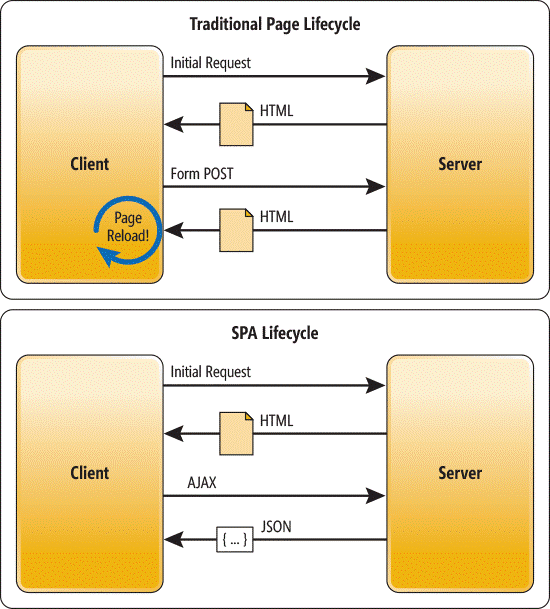
\includegraphics[scale=0.75]{spa.png}
  \caption{Жизненный цикл одностраничного приложения в сравнении с традиционным подходом}
  \label{figure:domain:spa}
\end{figure}

Преимущества одностраничных приложений:
\begin{itemize}
\item SPA характеризуются отличным быстродействием, так как большинство ресурсов, которые они используют (HTML+CSS+Скрипты), загружаются лишь однажды в течение сессии 
использования приложения. После совершения действий на странице меняются лишь данные.
\item Разработка веб-приложений обычно быстрее и эффективнее. Нет необходимости писать отдельный код для рендера страницы на стороне сервера. Также гораздо легче 
запустить процесс разработки подобных приложений, потому что писать код можно начинать с файла file://URI, не используя при этом никакой сервер.
\item SPA оптимизированы для Chrome debugging, разработчики могут отслеживать сетевые действия, изучать элементы страниц и данные, с ними ассоциируемые.
\item Если у вас уже есть SPA, будет возможность с тем же бэкендом создать и мобильное приложение.
\item SPA более эффективны в кэшировании данных на локальных носителях. Приложение высылает один запрос, собирает все необходимые данные, и с этого момента
 способно работать даже в режиме оффлайн.
\end{itemize}

Недостатки одностраничных приложений:
\begin{itemize}
\item SEO-оптимизация одностраничных приложений, по очевидным причинам, не очень проста. Контент приложений загружается при помощи AJAX (A-synchronous JavaScript and XML) -- метода
 обмена данными и обновления приложения без перезагрузки страницы, в то время как SEO-оптимизация основана на устойчивости контента в каждой отдельно взятой странице. При этом 
 продвижение вашего сайта в поисковиках не невозможно. Многие изменения в SEO можно провести на стороне сервера, а компании вроде Google продолжают придумывать новые решения для
 того, чтобы облегчить жизнь как владельцам SPA, так и их пользователям.
\item Они достаточно долго загружаются, поскольку тяжелые клиентские фреймворки должны сперва загрузиться в браузер.
\item SPA требуют JavaScript в активном режиме в браузерах пользователей. Если кто-то из ваших клиентов вручную отключит использование JavaScript, они не смогут в полной мере
воспользоваться вашим приложением. Даже если вы будете кэшировать и обрабатывать ваши страницы на стороне сервера (а это сейчас тоже возможно), вы всё ещё рискуете не доставить 
пользователям без JS все функции одностраничного приложения в правильном виде.
\item По сравнению с традиционными приложениями, SPA чуть хуже защищены. Благодаря межсайтовому скриптингу (XSS), злоумышленники имеют возможность внедрять дополнительные 
скрипты на стороне клиента.
\item Некоторые утечки памяти в JavaScript могут привести к падению производительности даже в мощных системах
 \end{itemize}

Исходя из вышеперечисленных преимущств и недостатков, можно заключить что SPA подходят для реализации приложений для редактирования некоторого пользовательского содержимого,
например для создания приложения для редактирования трехмерных моделей. Продолжительная работа с таким приложением не будет затруднена постоянными перезагрузками страниц, а
инкрементальное сохранение прогресса пользователя может быть реализовано в фоновом процессе.


\subsection{Особенности отображения 3D-графики в веб}
\label{sub:domain:overview_3d_in_web}
Основной особенностью отображения трехмерной графики в веб среде является невозможность прямого доступа к аппаратному обеспечению
посредством низкоуровневых графических библиотек, таких как OpenGL или Vulkan (Direct 3D в данной работе не рассматривается ввиду
проприетарности технологии) так как основная среда выполнения пользовательского кода в браузерах - виртуальная машина javascript,
не позволяющая пользовательскому коду использовать критические ресурсы компьютера.

Одной из технологий, позволяющей отображение трехмерной графики в браузере, является WebGL -- клиентская технология, построенная на базе
WebAssembly, платформы для разработки клиентских приложений с помощью native языков. WebAssembly -- также известный под названиями WA
или Wasm -- является платформой для выполнения низкоуровневого байт-кода, предназначенной для исполнения в браузере. В данный момент находится
на стадии разработки. Первоначальной целью была поддержка С/С++, хотя уже сейчас поддерживается Rust, и также в дальнейшем предполагается
поддержка других языков. WebAssemblу представляет собой переносимое абстрактное синтаксическое дерево, обеспечивающее как более быстрый парсинг,
так и более быстрое выполнение кода, чем JavaScript. Изначально WebAssembly основывался на asm.js и PNaCl. Команда, работающая над WebAssembly,
включает разработчиков из компаний Mozilla, Google, Microsoft и Apple, которые представляют на рынке четыре наиболее распространённых браузера — Firefox,
Chrome, Microsoft Edge и Safari соответственно.

WebGL — это контекст элемента canvas HTML, который обеспечивает API 3D графики без использования плагинов. Вся работа веб-приложений с использованием WebGL основана на коде JavaScript.
За счёт использования низкоуровневых средств поддержки OpenGL, часть кода на WebGL может выполняться непосредственно на видеокартах., благодаря чему разработчики могут получить доступ
к дополнительным ресурсам компьютера, увеличивая быстродействие работы приложений.
Таким образом, для создания приложений можно использовать стандартные для веб-среды технологии HTML/CSS/JavaScript и при этом также применять аппаратное ускорение графики.
Часто создание настольных приложений работающих с 2d и 3d-графикой нередко ограничивается возможностями целевой платформой, то здесь главным ограничением является только поддержка
браузером технологии WebGL. 
WebGL возник из экспериментов над Canvas 3D американского разработчика из компании Mozilla в 2006 году. Впоследствии разработчики браузеров Opera и Mozilla стали создавать свои
реализации WebGL. А впоследствии была организована рабочая группа с участием крупнейших разработчиков браузеров Apple, Google, Mozilla, Opera для работы над спецификацией
технологии. И в 3 марта 2011 года была представлена спецификация WebGL 1.0.

Использование WebAssembly позволяет пользовательскому коду, написанному на JavaScript потреблять API, реализованный низкоуровневыми библиотеками, реализованными
на языках C/C++ со скоростью, сравнимой со скоростью их выполнения в обычном приложении для рабочего стола. В дальшейнем, отрендеренную аппаратными средствами
текстуру можно отобразить на html5 canvas и интегрировать в веб-документ.

Для отображения трехмерной графики можно использовать один из нижеуказанных стеков технологий.
Для реализации логики приложения на основе стека Mono/.NET или cPython, можно использовать следующий подход:
\begin{enumerate}[label=\arabic*.]
\item Высокоуровневый движок рендеринга трехмерной графики, например Godot или Unity3D с поддержкой сборки для WebGL (\ref{figure:domain:webgl})
\item Unity/Godot WebPlayer для интерпретации логики приложения 
\item Библиотека трехмерной графики Three.js.
\item Реализация OpenGL для Web - WebGL.
\item WebAssembly и Emscripten для обращения к низкоуровневым графическим API OpenGL.
\item Реализация графического API OpenGL для C.
\end{enumerate}

\begin{figure}[ht]
\centering
  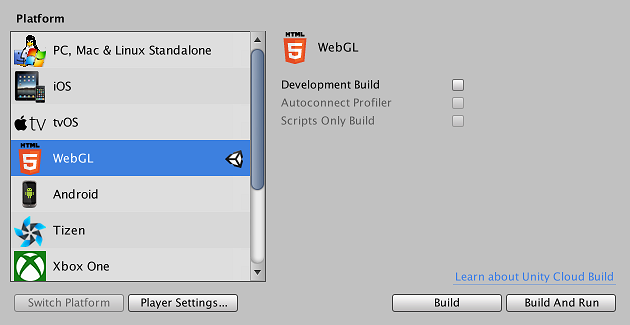
\includegraphics[scale=1.25]{webgl_build_unity.png}
  \caption{Инструменты для сборки Unity WebGL проекта}
  \label{figure:domain:webgl}
\end{figure}

Данный подход позволит реализовать одностраничное веб приложение, отображающее Godot или Unity3D проект в браузере, и по своей природе напоминает Flash-based SPA.
Для реализации веб приложения в виде классического веб сайта возможно использование того же стека технологий начиная с Three.js. В таком случае над графическим
приложением необходима реализация веб-приложения-обертки, которое разрабатывается на привычном для Web стеке технологий -- JavaScript, TypeScript, Dart:
\begin{enumerate}[label=\arabic*.]
\item Библиотека трехмерной графики Three.js а также управляющий приложением JavaScript или TypeScript код.
\item Реализация OpenGL для Web - WebGL.
\item WebAssembly и Emscripten для обращения к низкоуровневым графическим API OpenGL.
\item Реализация графического API OpenGL для C.
\end{enumerate}



\subsection{Краткий обзор фреймворка Reactjs}
\label{sub:domain:overview_spa_frameworks}
React (иногда React.js или ReactJS) — JavaScript-фреймворк с открытым исходным кодом для разработки пользовательских интерфейсов.

React разрабатывается и поддерживается Facebook, Instagram и сообществом отдельных разработчиков и корпораций.

React может использоваться для разработки одностраничных и мобильных приложений. Его цель — предоставить высокую скорость,
простоту и масштабируемость. В качетсве библиотеки для разработки пользовательских интерфейсов, React часто используется с другими библиотеками,
такими как Redux.

React был создан Джорданом Уокером, разработчиком програмного обеспечения из Facebook. На него оказал влияние XHP — компонентный HTML фреймворк для PHP.
В первый раз React был использован в новостной ленте Facebook в 2011 году и позже в ленте Instagram в 2012 году. Исходный код React был открыт в мае 2013
года на конференции «JSConf US».

React Native был анонсирован на конференции Facebook «React.js Con» в феврале 2015 года, а исходный код был открыт в марте 2015 года. Он позволяет
разрабатывать нативные Android, iOS и UWP приложения с использованием React.

18 апреля 2017 года Facebook анонсировал React Fiber, переписанную и оптимизированную версию React. React Fiber станет основой разработки всех
будущих функций и улучшений.

Ниже приведен пример использования React в HTML с JSX и JavaScri-pt.

\begin{lstlisting}[language=HTML, label=lst:domain:reactjs]
<div id="myReactApp"></div>

<script type="text/babel">
  
  class Greeter extends React.Component { 
    
    render() { 
      return <h1>{this.props.greeting}</h1>
    } 

  } 

  ReactDOM.render(
      <Greeter greeting="Hello World!" />,
      document.getElementById('myReactApp')
  );

</script>
\end{lstlisting}

Класс Greeter это React компонент, который принимает свойство gree-ting. Метод ReactDOM.render отрисовывает
экземпляр класса (компонента) Greeter с свойством greeting равным 'Hello World' и вставляет отрисованный компонент в
DOM-элемент с идентификатором myReactApp как вложенный элемент.

При отображении в веб-браузере, результат будет

\begin{lstlisting}[language=HTML, label=lst:domain:html]
<div id="myReactApp">
  <h1>
    Hello World!
  </h1>
</div>
\end{lstlisting}

В контексте данной работы, фреймворк Reactjs можно применить для реализации пользовательского интерфейса приложения-обертки
над компонентами WebGL. Поскольку реализация стандартных механизмов валидации компонентов пользовательского интерфейса может
быть затруднительна, а основная часть работ при реализации любого приложения-редактора -- дизайн и создание пользовательского
интерфейса, целесообразно использовать стандартные возможности HTML/CSS для проектирования пользовательского интерфейса и
использование парадигмы Redux с функциональным подходом к разработке кода для создания системы основанной на централизованном
хранилище состояния.

Для упрощения взаимодействия между компонентами системы предлагается использование парадигмы Redux. Redux -- система для управления
состоянием в приложении. Поддерживает возможность реализации полностью функционального кода, избавляя приложение от необходимости
ручной мутации состояния, преобразуя его в канонический автомат Мили.

Функции переходов такого автомата реализуются с помощью так называемых модулей-Reducer'ов (отсюда и название библиотеки), а состояние
в любой момент времени определяется как применение того или иного Reducer'а к текущему состоянию. Определение подходящей ветки
работы Reducer'а производится исходя из типа действия, выполняемого пользователем в приложении.

Поскольку подобная система является абсолютно чистой с точки зрения мутации данных в приложении, становится возможна реализация
сохранения истории работы пользователя, а так же, ввиду обратимости всех чистых изменений или возможности сохранения истории
<<снимков состояния>> приложения, возможно просто реализовать механизм отката произвольного количества действий пользователя.

На такую систему, однако, накладывается ряд ограничений:

\begin{enumerate}[label=\arabic*.]
\item Все изменения должны быть строго детерменированы, то есть не допускается использование модуля Random.
\item В системе должен быть один источник состояния, называемый Data Store
\item Все промежуточное состояние приложения должно следовать по пути от высокоуровневого компонента иерархии к низкоуровневым.
\end{enumerate}

\begin{figure}[ht]
\centering
  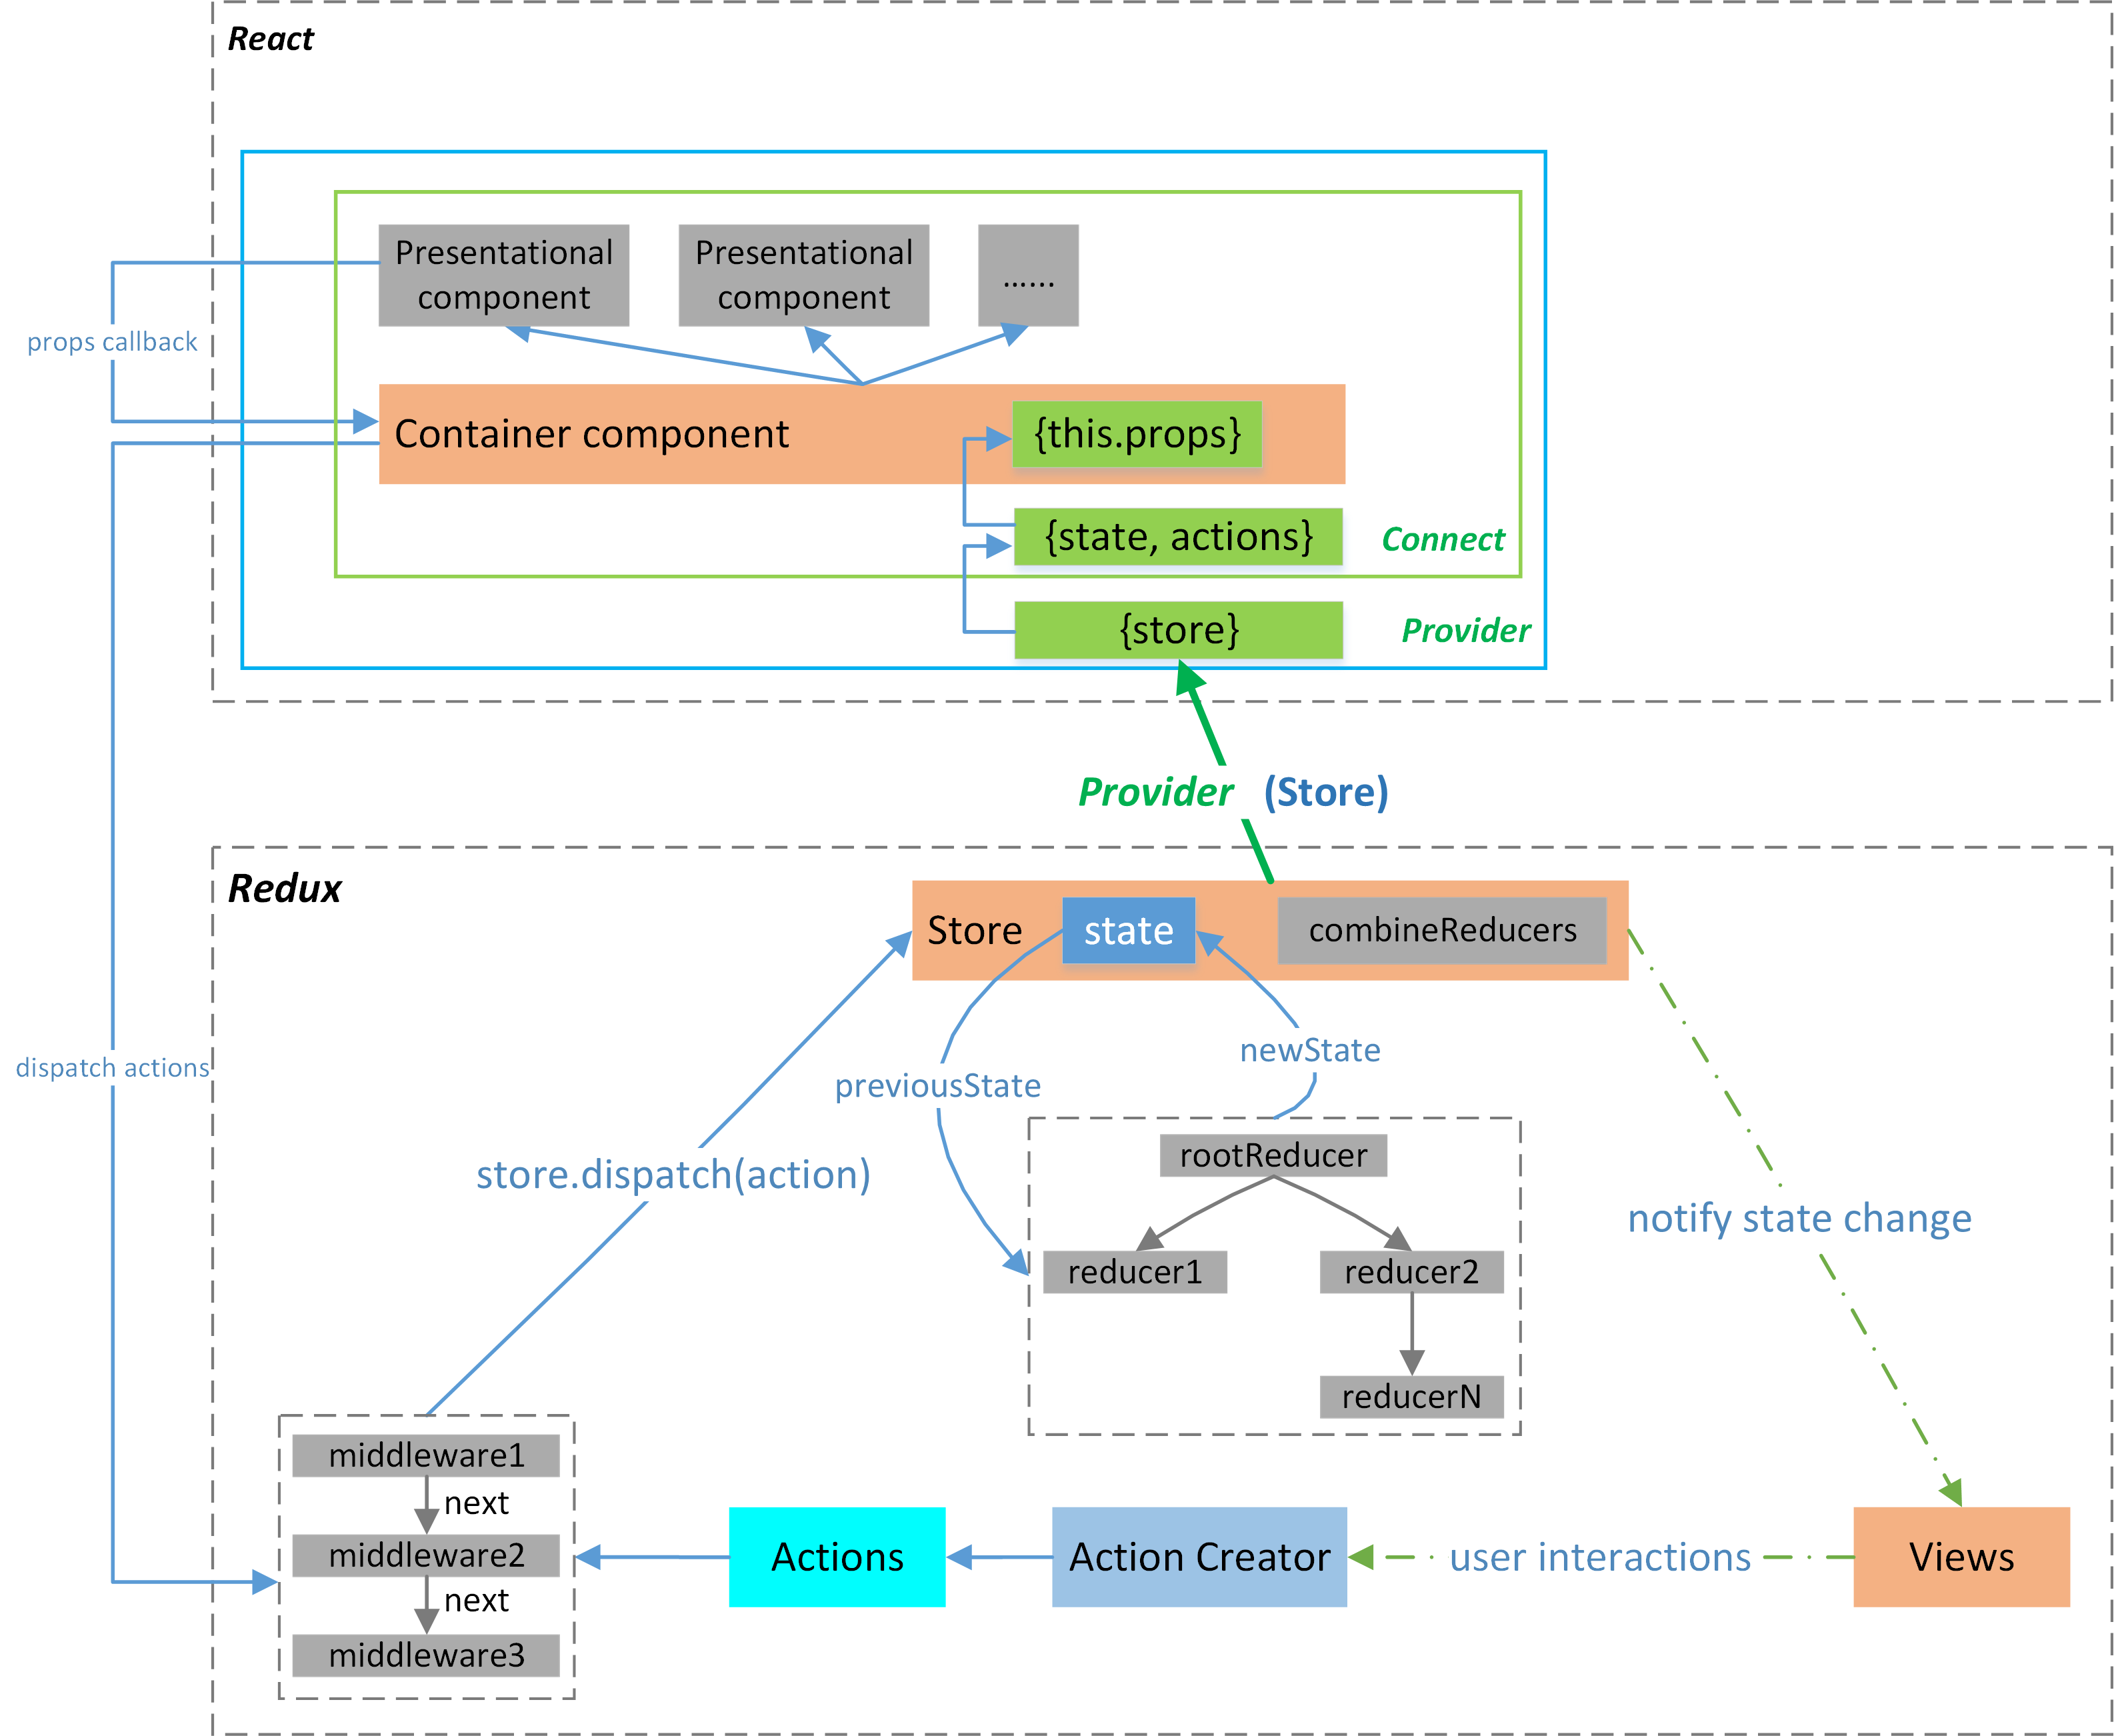
\includegraphics[scale=0.80]{react_redux.png}
  \caption{Диаграмма взаимодействия компонентов в React-Redux приложении}
  \label{figure:domain:react_redux}
\end{figure}

Жизненный цикл Redux-приложения заключается в следующих четырех шагах:

\begin{enumerate}[label=\arabic*.]
\item
 Вызов метода store.dispatch(action)
 Аргумент action содержит метаинформацию о типе действия, произведенного пользователем. Действия могут быть описаны следующими JSON-объектами:
 \begin{lstlisting}[language=TypeScript, label=lst:domain:redux0]
 {
  type: 'LIKE_ARTICLE',
   articleId: 42
 }

 {
   type: 'FETCH_USER_SUCCESS',
   response: {
     id: 3,
     name: 'Mary'
   }
 }

 {
   type: 'ADD_TODO',
   text: 'Read the Redux docs.'
 }
 \end{lstlisting}
 Действия могут быть иницированны из любой точки приложения, имеющий доступ к центральному хранилищу состояния, включая всевозможные компоненты, события XHR, запланированные интервалы.

\item
  Вызов reduce-метода хранилищем состояния. Reduce-метод имеет следующую сигнатуру:
  \begin{lstlisting}[language=TypeScript, label=lst:domain:redux1]
    (Si, Ai) => Si+1
  \end{lstlisting}

  Примером типичного reduce-метода может служить следующий метод из классического 

  \begin{lstlisting}[language=TypeScript, label=lst:domain:redux2]
  let previousState = {
    visibleTodoFilter: 'SHOW_ALL',
    todos: [
      {
        text: 'Read the docs.',
        complete: false
      }
    ]
  }

  let action = {
    type: 'ADD_TODO',
    text: 'Understand the flow.'
  }

  let nextState = todoApp(previousState, action)

  \end{lstlisting}

  Reducer-метод является чистой функцией, то есть он лишь вычисляет новое состояние. Функция-reducer должна быть абсолютно детерменированной:
  вызое ее с одними и теми же аргументами обязан всегда производить точно такие-же результаты, а так-же не должен сопровождаться побочными эффектами,
  такими как изменение маршрута веб-приложения, вызова сторонних API. Все подобные изменения должны производиться до того как действия вызываются.

\item
  Корневая reduce-функция может комбинировать результаты нескольких дочерних reduce-функций для получения полного состояния системы после произведения пользовательских операций.
  Стандартный метод комбинирования reduce-функций - вспомогательный метод combineReducers(), предоставляемый Redux. Ниже указан пример использования combineRedu-cers:

  \begin{lstlisting}[language=TypeScript, label=lst:domain:redux3] 
  function todos(state = [], action) {
    return nextState;
  }

  function visibleTodoFilter(
    state = 'SHOW_ALL',
    action)
  {
    return nextState;
  }

  let todoApp = combineReducers({
    todos,
    visibleTodoFilter
  });

 \end{lstlisting}

 Таким образом, когда пользователь производит действие, будет вызвана комбинация двух reduce-методов, что,
 однако, не приводит к гонкам из-за отсутствия в них побочных дейстивий:
 
 \begin{lstlisting}[language=TypeScript, label=lst:domain:redux4]
 let nextTodos = todos(state.todos, action)
 let nextVisibleTodoFilter =>
   visibleTodoFilter(state.visibleTodoFilter, action)

 return {
    todos: nextTodos,
    visibleTodoFilter: nextVisibleTodoFilter
  }
 \end{lstlisting}

\item
 Reduce-метод сохраняет состояние системы в хранилище состояния и вызвает перерисовку пользовательского интерфейса посредством вызова всех событий, на которые подписана UI система:

 \begin{lstlisting}[language=TypeScript, label=lst:domain:redux5]
   onComponentDidMount: () => {
     store.subscribe((newState) =>
       component.setState(newState)
     );
   } 
 \end{lstlisting}

\end{enumerate}


% - Как ее можно применить в веб среде
% - Целесообразно ли это
% - Как можно перенести процесс создания 3д графики в веб
% - Обзор подходов и технологий 3д графики в веб среде